\documentclass{beamer}

%
% Choose how your presentation looks.
%
% For more themes, color themes and font themes, see:
% http://deic.uab.es/~iblanes/beamer_gallery/index_by_theme.html
%
\mode<presentation>
{
  \usetheme{default}      % or try Darmstadt, Madrid, Warsaw, ...
  \usecolortheme{default} % or try albatross, beaver, crane, ...
  \usefonttheme{default}  % or try serif, structurebold, ...
  \setbeamertemplate{navigation symbols}{}
  \setbeamertemplate{caption}[numbered]
  \setbeamertemplate{footline}[page number]
  \setbeamercolor{frametitle}{fg=white}
  \setbeamercolor{footline}{fg=black}
} 

\usepackage[english]{babel}
\usepackage[utf8x]{inputenc}
\usepackage{tikz}
\usepackage{listings}
\usepackage{courier}

\xdefinecolor{darkblue}{rgb}{0.1,0.1,0.7}
\xdefinecolor{dianablue}{rgb}{0.18,0.24,0.31}
\definecolor{commentgreen}{rgb}{0,0.6,0}
\definecolor{stringmauve}{rgb}{0.58,0,0.82}

\lstset{ %
  backgroundcolor=\color{white},      % choose the background color
  basicstyle=\ttfamily\small,         % size of fonts used for the code
  breaklines=true,                    % automatic line breaking only at whitespace
  captionpos=b,                       % sets the caption-position to bottom
  commentstyle=\color{commentgreen},  % comment style
  escapeinside={\%*}{*)},             % if you want to add LaTeX within your code
  keywordstyle=\color{blue},          % keyword style
  stringstyle=\color{stringmauve},    % string literal style
  showstringspaces=false,
  showlines=true
}

\lstdefinelanguage{scala}{
  morekeywords={abstract,case,catch,class,def,%
    do,else,extends,false,final,finally,%
    for,if,implicit,import,match,mixin,%
    new,null,object,override,package,%
    private,protected,requires,return,sealed,%
    super,this,throw,trait,true,try,%
    type,val,var,while,with,yield},
  otherkeywords={=>,<-,<\%,<:,>:,\#,@},
  sensitive=true,
  morecomment=[l]{//},
  morecomment=[n]{/*}{*/},
  morestring=[b]",
  morestring=[b]',
  morestring=[b]"""
}

\title[2016-05-19-uscms-diana]{The DIANA-HEP Project}
\author{Jim Pivarski}
\institute{Princeton University}
\date{May 19, 2016}

\begin{document}

\logo{\pgfputat{\pgfxy(0.11, 8)}{\pgfbox[right,base]{\tikz{\filldraw[fill=dianablue, draw=none] (0 cm, 0 cm) rectangle (50 cm, 1 cm);}}}\pgfputat{\pgfxy(0.11, -0.6)}{\pgfbox[right,base]{\tikz{\filldraw[fill=dianablue, draw=none] (0 cm, 0 cm) rectangle (50 cm, 1 cm);}
\includegraphics[height=0.99 cm]{diana-hep-logo.png}\tikz{\filldraw[fill=dianablue, draw=none] (0 cm, 0 cm) rectangle (4.9 cm, 1 cm);}}}}

\begin{frame}
  \titlepage
\end{frame}

\logo{\pgfputat{\pgfxy(0.11, 8)}{\pgfbox[right,base]{\tikz{\filldraw[fill=dianablue, draw=none] (0 cm, 0 cm) rectangle (50 cm, 1 cm);}
\includegraphics[height=1 cm]{diana-hep-logo.png}}}}

% Uncomment these lines for an automatically generated outline.
%\begin{frame}{Outline}
%  \tableofcontents
%\end{frame}

\begin{frame}{What is DIANA-HEP?}

\begin{block}{}
\vspace{-0.25 cm}
DIANA is a project to develop state-of-the-art cross-experiment analysis software.

\vspace{0.25 cm}
\begin{uncoverenv}<2->
Not a (single) software product, but a collaborative project to extend software as sustainable infrastructure and improve:
\begin{itemize}
\item \textcolor{darkblue}{performance:} ROOT I/O, vectorization, parallelization
\item \textcolor{darkblue}{interoperability:} Scientific Python ecosystem, the Big Data ecosystem (Hadoop, Spark), statistical packages in R
\item \textcolor{darkblue}{reproducibility:} RooFit workspace, HEPdata, CAP
\end{itemize}
\end{uncoverenv}
\end{block}

\begin{uncoverenv}<3->
\begin{block}{Funding}
\begin{itemize}
\item Part of NSF's Software Infrastructure for Sustained Innovation
\item Four years, 6--7 FTE spread over four universities \\ (Princeton, NYU, Cincinnati, U.\ Nebraska-Lincoln)
\end{itemize}
\end{block}
\end{uncoverenv}
\end{frame}

\begin{frame}{$(\mbox{SI})^2$}
\vspace{0.4 cm}

\includegraphics[width=\linewidth]{si2_cover.png}
\end{frame}

%% \begin{frame}{$(\mbox{SI})^2$}
%% \vspace{0.4 cm}
%% 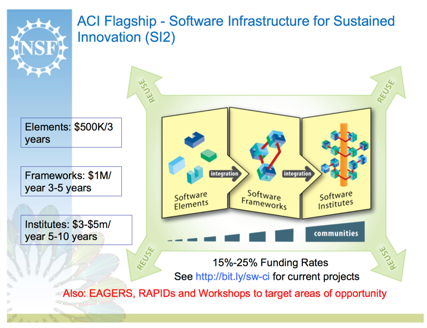
\includegraphics[width=\linewidth]{si2_puzzle.png}
%% \end{frame}

\begin{frame}{$(\mbox{SI})^2$}
\vspace{0.75 cm}
\mbox{ } \hfill \mbox{\hspace{0.4 cm}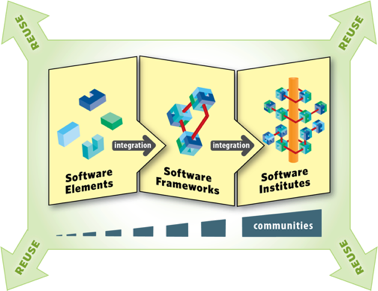
\includegraphics[height=4 cm]{puzzle.png}\hspace{-0.4 cm}}

\vspace{-4 cm}
\begin{enumerate}
\item {\bf Scientific Software \\ Elements (SSE)} awards for \\ small groups to create and \\ deploy Software Elements.
\item {\bf Scientific Software \\ Integration (SSI)} awards are \\ for larger, interdisciplinary \\ teams organized around \\ developing Software Frameworks.
\item {\bf Scientific Software Innovation Institutes (S2I2)} awards are for establishing long-term hubs that will serve a large research community.
\end{enumerate}

\begin{center}
\textcolor{darkblue}{DIANA-HEP is a Scientific Software Integration (SSI)}
\end{center}
\end{frame}

%% \begin{frame}{Principle Investigators}
%% \scriptsize

%% \vfill

%% \begin{columns}[t]
%% \column{0.5\linewidth}
%% \textcolor{darkblue}{Peter Elmer (Princeton)}
%% \begin{columns}
%% \column{0.25\linewidth}
%% 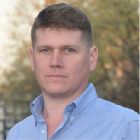
\includegraphics[height=2 cm]{peter_elmer.png}
%% \column{0.75\linewidth}
%% \begin{itemize}
%% \item Many roles in Software/Computing in BaBar and CMS
%% \item Early involvement in xrootd, etc.
%% \end{itemize}
%% \end{columns}

%% \column{0.5\linewidth}
%% \textcolor{darkblue}{Mike Sokoloff (Cincinnati)}
%% \begin{columns}
%% \column{0.25\linewidth}
%% 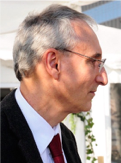
\includegraphics[height=2 cm]{mike_sokoloff.png}
%% \column{0.75\linewidth}
%% \begin{itemize}
%% \item Flavor analysis on BaBar/LHCb
%% \item NSF-funded R\&D investigation into many/multicore: GooFit prototype, likelihood fitting
%% \end{itemize}
%% \end{columns}
%% \end{columns}

%% \vfill
%% \begin{columns}[t]
%% \column{0.5\linewidth}
%% \textcolor{darkblue}{Brian Bockelman (U. Nebraska-Lincoln)}
%% \begin{columns}
%% \column{0.25\linewidth}
%% 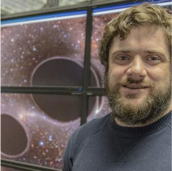
\includegraphics[height=2 cm]{brian_bockelman.png}
%% \column{0.75\linewidth}
%% \begin{itemize}
%% \item Computer Science research faculty
%% \item CMS and Tier2 Computing and Open Science Grid
%% \item NSF-funded AAA project (xrootd-based data federation)
%% \item I/O performance research
%% \end{itemize}
%% \end{columns}

%% \column{0.5\linewidth}
%% \textcolor{darkblue}{Kyle Cranmer (NYU)}
%% \begin{columns}
%% \column{0.25\linewidth}
%% 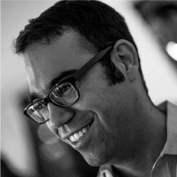
\includegraphics[height=2 cm]{kyle_cranmer.png}
%% \column{0.75\linewidth}
%% \begin{itemize}
%% \item ATLAS physics research
%% \item RooStats and HistFactory, statistical procedures and Higgs combination
%% \item RECAST, \mbox{data preservation\hspace{-0.5 cm}} (NSF-funded DASPOS), Moore-Sloan Data Science Environment
%% \end{itemize}
%% \end{columns}
%% \end{columns}
%% \end{frame}

\begin{frame}{DIANA Project team}
\scriptsize
\begin{description}
\item[Peter Elmer] (lead PI) Princeton, CMS
\item[Brian Bockelman] (PI) U.\ Nebraska-Lincoln, CMS
\item[Kyle Cranmer] (PI) NYU, ATLAS
\item[Mike Sokoloff] (PI) Cincinnati, LHCb
\item[Jinyang Li] (Senior Personnel) NYU, Computer Science Department
\item[David Lange] Princeton, CMS co-coordinator of Offline Software and Computing
\item[Gilles Louppe] NYU, ATLAS, Machine learning Ph.D.\ (former CERN fellow), scikit-learn developer
\item[Jim Pivarski] Princeton, CMS, interoperability of Hadoop/Spark with ROOT/CMSSW
\item[Eduardo Rodigues] Cincinnati, LHCb, coordinator analysis tools, tracking, trigger, fitting
\item[Zhe Zhang] Nebraska, Computer Science Ph.D.\ student, improving I/O performance
\item[Chien-Chin Huang] NYU, Computer Science Ph.D.\ student, RooFit data parallelism, Theano, TensorFlow, etc.
\end{description}
\end{frame}

\begin{frame}{Principle Investigators}
\hspace{-0.6 cm}\textcolor{darkblue}{\large Peter Elmer (Princeton)}

\vspace{0.25 cm}
\begin{columns}
\column{0.125\linewidth}
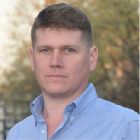
\includegraphics[height=2 cm]{peter_elmer.png}

\column{0.875\linewidth}
\begin{itemize}
\item Many roles in Software/Computing in BaBar \& CMS
\item Early involvement in xrootd, etc.
\end{itemize}
\end{columns}

\vspace{1 cm}
\hspace{-0.6 cm}\textcolor{darkblue}{\large Mike Sokoloff (Cincinnati)}

\vspace{0.25 cm}
\begin{columns}
\column{0.125\linewidth}
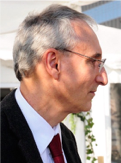
\includegraphics[height=2 cm]{mike_sokoloff.png}

\column{0.875\linewidth}
\begin{itemize}
\item Physics research: flavor analysis on BaBar/LHCb
\item NSF-funded R\&D investigation into many/multicore: GooFit prototype, likelihood fitting
\end{itemize}
\end{columns}
\end{frame}

\begin{frame}{Principle Investigators}
\hspace{-0.6 cm}\textcolor{darkblue}{\large Brian Bockelman (U.\ Nebraska-Lincoln)}

\begin{columns}
\column{0.125\linewidth}
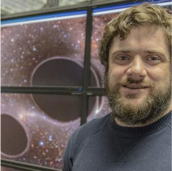
\includegraphics[height=2 cm]{brian_bockelman.png}

\column{0.875\linewidth}
\begin{itemize}
\item Computer Science research faculty
\item CMS and Tier2 Computing and Open Science Grid
\item NSF-funded AAA (xrootd-based data federation)
\item Collaboration on I/O system: initially performance on long-latency systems, leading also to general purpose improvements/contributions
\end{itemize}
\end{columns}

\vspace{0.25 cm}
\hspace{-0.6 cm}\textcolor{darkblue}{\large Kyle Cranmer (NYU)}

\begin{columns}
\column{0.125\linewidth}
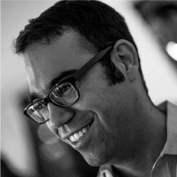
\includegraphics[height=2 cm]{kyle_cranmer.png}

\column{0.875\linewidth}
\begin{itemize}
\item ATLAS physics research
\item RooStats and HistFactory, statistical procedures and Higgs combination
\item RECAST, data preservation (NSF-funded DASPOS), Moore-Sloan Data Science Environment
\end{itemize}
\end{columns}
\end{frame}

\begin{frame}{Gilles Louppe (NYU)}
\mbox{ } \hfill 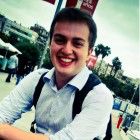
\includegraphics[height=2 cm]{gilles_louppe.png}

\vspace{-2 cm}
\begin{itemize}
\item Computer science background, postdoc in \\ machine learning, scikit-learn core developer
\item Development of machine learning software and \\ applications to HEP
\begin{itemize}
\item carl: likelihood-free inference toolbox
\item scikit-optimize: user-friendly toolbox for black box optimization
\end{itemize}

\item Machine learning research, targeted to HEP use-cases
\begin{itemize}
\item likelihood-free classifiers
\item ATLAS projects
\end{itemize}

\item Education: various courses, tutorials, and talks given on machine learning and related software
\end{itemize}
\end{frame}

\begin{frame}{Eduardo Rodrigues (Cincinnati)}
\mbox{ } \hfill 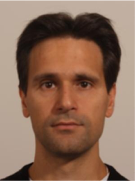
\includegraphics[height=2 cm]{eduardo_rodrigues.png}

\vspace{-2 cm}
\begin{itemize}
\item LHCb physicist since 2002
\item Coordinator of Physics Analysis Software Project
\item Convener of Physics Working Group on Charmless \\ $b$-hadron Decays
\item Vertex Software Coordinator
\end{itemize}

\vspace{0.25 cm}
\begin{itemize}
\item Goals: to make sure that software meets physicists' requirements, physicsts get to use the best tools available and/or being developed
\item Particular interes in machine learning related software
\item Keen on tutorials, e.g.\ gave a course on RooFit in 2012
\end{itemize}
\end{frame}

\begin{frame}{Jim Pivarski (Princeton)}
\mbox{ } \hfill 
\includegraphics[height=2 cm]{jim_pivarski.png}

\vspace{-2 cm}
\begin{itemize}
\item Physics: 5 years at CLEO, 5 years commissioning \\ CMS Run I (muon alignment)
\item Industry: 5 years as a data science consultant, \\ helping small and large companies with data \\ analysis techniques and Big Data software
\item Created language-agnostic standard for encoding data mining models that has been adopted by the \mbox{industry (\textcolor{blue}{\small \url{dmg.org/pfa}})\hspace{-1 cm}}
\item DIANA focus:
\begin{enumerate}
\item integrating physics analyses with Big Data software
\item introducing physicists to more high-level and function styles of data analysis
\item creating tools that bridge both worlds
\end{enumerate}
\end{itemize}
\end{frame}

\begin{frame}{David Lange (Princeton)}
\vspace{0.25 cm}
\mbox{ } \hfill 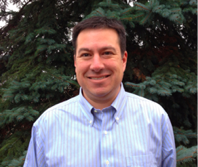
\includegraphics[height=2 cm]{david_lange.png}

\vspace{-2 cm}
\begin{itemize}
\item Many software roles in BaBar and CMS
\item Original co-author of EvtGen
\item Currently CMS offline/computing \\ co-coordinator until September 2016
\item Near-term DIANA goals: investigating interoperability between Python and ROOT
\end{itemize}

\vspace{1.25 cm}
\pgfputat{\pgfxy(20, 0)}{\pgfbox[right,base]{\tikz{\filldraw[fill=dianablue, draw=none] (0 cm, 0 cm) rectangle (50 cm, 1 cm);}}}

\vspace{-0.3 cm}
\hspace{-0.83 cm} \textcolor{white}{\Large TBN: (U.\ Nebraska-Lincoln)}

\vspace{0.25 cm}
\mbox{ } \hfill 
\includegraphics[height=2 cm]{guy_fawkes.png}

\vspace{-2 cm}
\begin{itemize}
\item One staff position is still being filled\ldots
\end{itemize}
\end{frame}

\begin{frame}{DIANA Fellows}
\begin{block}{Graduate Fellows}
Four per year; three months intensively developing tools with collaborating institutions.
\begin{itemize}
\item call for applications will go out soon
\end{itemize}
\end{block}

\vfill
\begin{block}{Undergraduate Fellow}
One for 10--12 weeks in the summer, either developing or using data-intensive tools.
\end{block}
\end{frame}

\begin{frame}{DIANA topical meetings}
\begin{columns}
\column{0.5\linewidth}
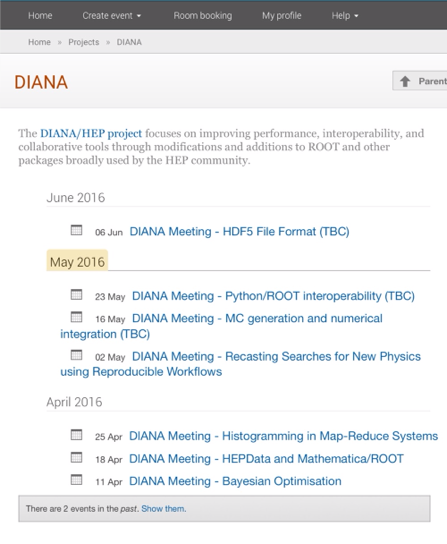
\includegraphics[width=\linewidth]{topical_meetings.png}

\column{0.5\linewidth}
\begin{itemize}\setlength{\itemsep}{0.3 cm}
%% \item Forum for discussion about analysis techniques
%% \item Explore near-term and long-term possibilities, ideas, and collaboration
\item Engage people from multiple experiments and from beyond HEP
\item Steady state: expect 2 meetings per month
\item If you have ideas, please contact us!
\end{itemize}
\end{columns}
\end{frame}

\begin{frame}{GitHub organization}
\vspace{0.5 cm}
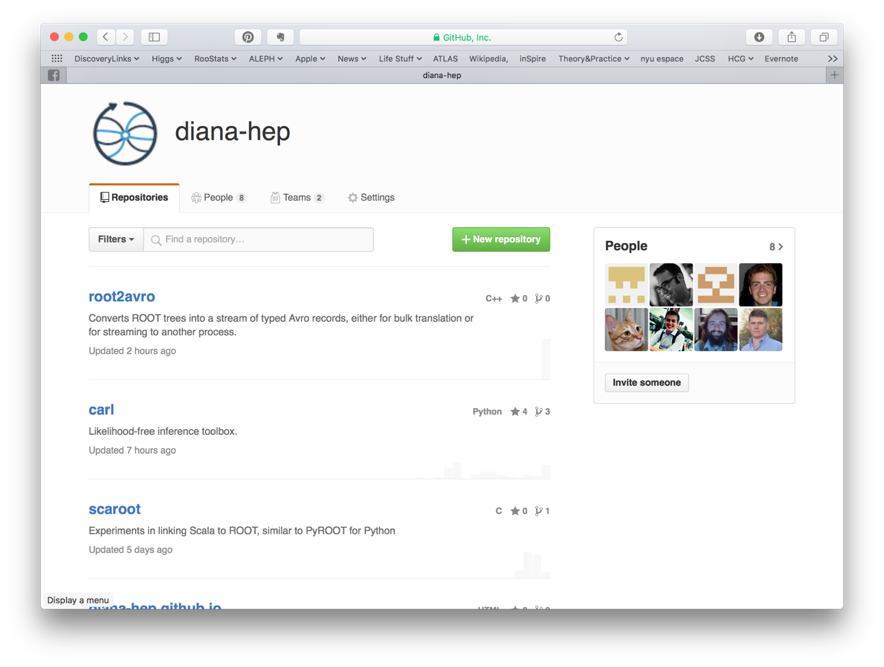
\includegraphics[width=\linewidth]{github_organization.png}
\end{frame}

\begin{frame}{My own work}
\vspace{2.5 cm}
\mbox{ } \hfill {\hspace{0.6 cm}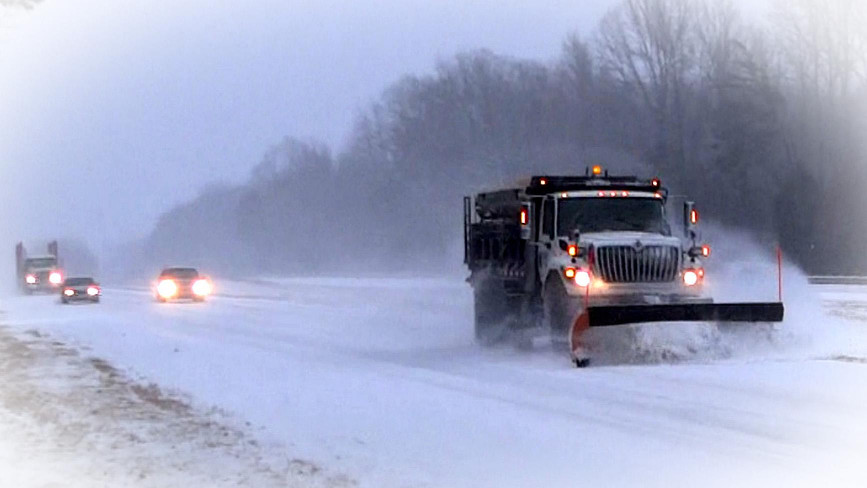
\includegraphics[height=2.5 cm]{snowplow.jpg}\hspace{-0.6 cm}}

\vspace{-4.7 cm}
I've been helping an analysis group port their dark matter search from custom C++ to Apache Spark:
\begin{itemize}
\item Oliver Gutsche, Matteo Cremonesi, Cristina Su\'arez
\item Part of a wider effort, including \\ Alexey Svyatkovskiy (Princeton), \\ Saba Sehrish and Jim Kowalkowski \\ (FNAL Scientific Computing)
\item Resolving technical issues before \\ the analyzers hit them\ldots
\end{itemize}

\vspace{0.3 cm}
\begin{uncoverenv}<2->
\mbox{ } \hfill 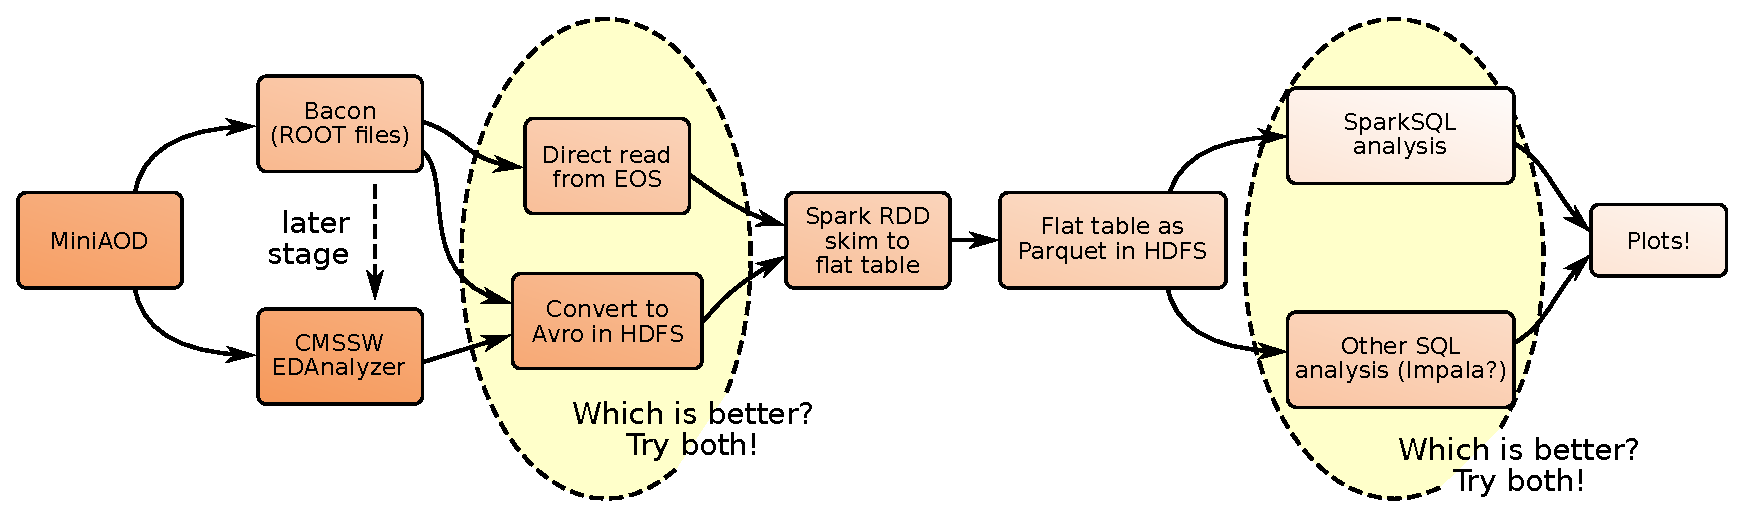
\includegraphics[width=0.8\linewidth]{spark_workflow.pdf} \hfill \mbox{ }
\end{uncoverenv}
\end{frame}

\begin{frame}{My own work}
\setbeamercolor{normal text}{fg=gray,bg=}
\setbeamercolor{alerted text}{fg=black,bg=}
\usebeamercolor{normal text}
\vspace{0.25 cm}
\begin{itemize}
\item<1-> \alert<1>{Reading complex data structures from ROOT:}
\begin{itemize}
\item \alert<1>{TTrees containing arbitrary C++ classes (whole events)}
\item \alert<1>{to Avro (schemaed, binary JSON), Parquet (columnar store)}
\item \alert<1>{directly into Spark (in Java Virtual Machine (JVM))}
\end{itemize}

\item<2-> \alert<2>{Generic access to C++ and ROOT from JVM}
\begin{itemize}
\item \alert<2>{write API in Java or Scala, implementation in C++}
\end{itemize}

\item<3-> \alert<3-7>{Histogram aggregation in a functional paradigm}
\begin{itemize}
\item<4-> \alert<4-7>{a better fit to Spark's functional workflows}
\item<5-> \alert<5-7>{exports to ROOT, Matplotlib, etc., rather than reimplementing plotting code}
\item<6-> \alert<6-7>{side-effect of formalizing analysis:}
\begin{uncoverenv}<6->
\begin{itemize}
\item \alert<6-7>{automatically identify which cuts are applied to each plot}
\item \alert<6-7>{more robust against modifications (e.g.\ unit changes)}
\end{itemize}
\end{uncoverenv}
\item<7-> \alert<7>{small framework can aggregate data in hard-to-reach places, such as GPU code, awk-like quick plots}
\end{itemize}

\item<8-> \alert<8>{Transpile restricted Python to low-level backends (future)}
\begin{itemize}
\item \alert<8>{key is to identify restrictions that give optimizer strong assumptions, but leave enough capabilities for physics code\ldots}
\end{itemize}
\end{itemize}
\end{frame}

\begin{frame}{Summary/Overview}
\vspace{0.5 cm}
\begin{columns}
\column{1.15\linewidth}
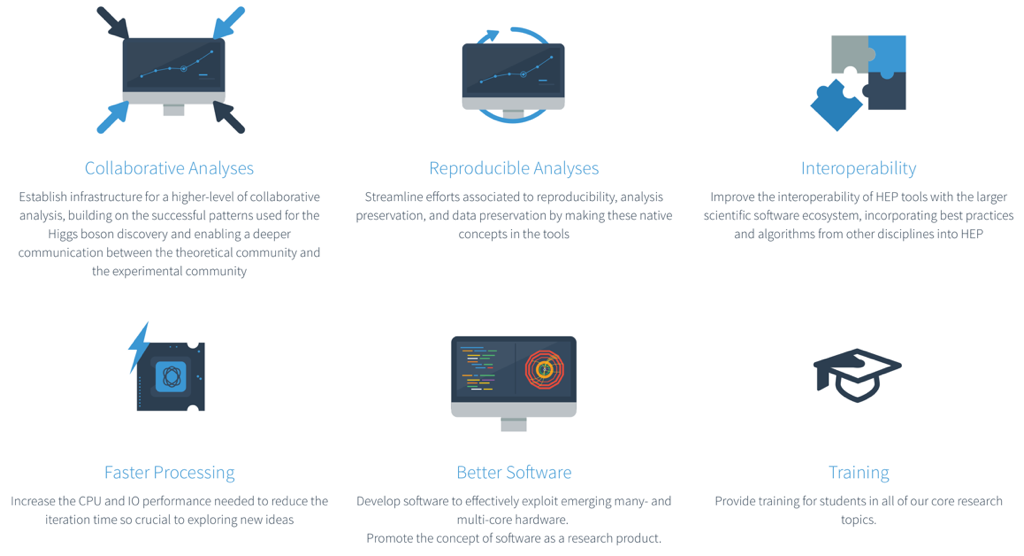
\includegraphics[width=\linewidth]{diana_goals.png}
\end{columns}
\end{frame}

\end{document}
